\documentclass[]{article}
%\usepackage{lmodern}
\usepackage{amssymb,amsmath}
\usepackage{ifxetex,ifluatex}
\usepackage{fixltx2e} % provides \textsubscript
\ifnum 0\ifxetex 1\fi\ifluatex 1\fi=0 % if pdftex
  \usepackage[T1]{fontenc}
  \usepackage[utf8]{inputenc}
\else % if luatex or xelatex
  \ifxetex
    \usepackage{mathspec}
    \usepackage{xltxtra,xunicode}
  \else
    \usepackage{fontspec}
  \fi
  \defaultfontfeatures{Mapping=tex-text,Scale=MatchLowercase}
  \newcommand{\euro}{€}
\fi
% use upquote if available, for straight quotes in verbatim environments
\IfFileExists{upquote.sty}{\usepackage{upquote}}{}
% use microtype if available
\IfFileExists{microtype.sty}{%
\usepackage{microtype}
\UseMicrotypeSet[protrusion]{basicmath} % disable protrusion for tt fonts
}{}
\usepackage{graphicx}
\makeatletter
\def\maxwidth{\ifdim\Gin@nat@width>\linewidth\linewidth\else\Gin@nat@width\fi}
\def\maxheight{\ifdim\Gin@nat@height>\textheight\textheight\else\Gin@nat@height\fi}
\makeatother
% Scale images if necessary, so that they will not overflow the page
% margins by default, and it is still possible to overwrite the defaults
% using explicit options in \includegraphics[width, height, ...]{}
\setkeys{Gin}{width=\maxwidth,height=\maxheight,keepaspectratio}
\ifxetex
  \usepackage[setpagesize=false, % page size defined by xetex
              unicode=false, % unicode breaks when used with xetex
              xetex]{hyperref}
\else
  \usepackage[unicode=true]{hyperref}
\fi
\hypersetup{breaklinks=true,
            bookmarks=true,
            pdfauthor={},
            pdftitle={Pessimism},
            colorlinks=true,
            citecolor=blue,
            urlcolor=blue,
            linkcolor=magenta,
            pdfborder={0 0 0}}
\urlstyle{same}  % don't use monospace font for urls
\setlength{\parindent}{0pt}
\setlength{\parskip}{6pt plus 2pt minus 1pt}
\setlength{\emergencystretch}{3em}  % prevent overfull lines
\setcounter{secnumdepth}{0}

\title{Pessimism}
\date{}

\begin{document}
\maketitle

\section{Does life have any meaning?}\label{does-life-have-any-meaning}

\subsection{Personal Note}\label{personal-note}

We will be talking about death, suicide, and depression in this module.
These are uncomfortable topics for many and have touched most of us
directly or indirectly. They raise core philosophical questions, perhaps
raise the most important philosophical questions. I would like to
encourage you to keep a very open mind about the material. A full and
proper study of the issues would take many years. You might also like to
know that NJCU offers \href{http://www.njcu.edu/counselingcenter}{free
counseling services} to registered NJCU students.

\subsection{Introduction}\label{introduction}

You are mortal. Your friends, families, and loved ones are mortal. Each
of us will die. It is easy to ignore it. We often think of death as
happening some point in the far future. Like a distant land that we may
have to visit one day, that land is not this land and we prefer not
thinking about it. Unfortunately, death is an ever pressing possibility.
Several have recently died from Legionnaires disease in the Bronx. Many
are killed in car accidents every day. There are the bizarre accidents
too. You don't think that this might be the day you die. It's too
depressing! But you could die at any moment. You might stumble and hit
your head awkwardly. A wall might collapse upon you.

In this module, we are going to examine Leo Tolstoy's argument that our
mortality robs our life of meaning, though, we will also look at the
meaning he did finally find in life. Tolstoy puts his concern as
follows:

\begin{quote}
\ldots{} My question - that which at the age of fifty brought me to the
verge of suicide - was the simplest of questions, lying in the soul of
every man from the foolish child to the wisest elder: it was a question
without an answer to which one cannot live, as I had found by
experience. It was: ``What will come of what I am doing today or shall
do tomorrow? What will come of my whole life?'' (Tolstoy, p.14)
\footnote{Tolstoy, Leo, \href{/Teaching/Examined/Meaning/Tolstoy.pdf}{`A
  Confession'}, 1882}
\end{quote}

\begin{quote}
Differently expressed, the question is: ``Why should I live, why wish
for anything, or do anything?'' It can also be expressed thus: ``Is
there any meaning in my life that the inevitable death awaiting me does
not destroy? (Tolstoy, p.14)
\end{quote}

This handout proceeds in the two parts. The first clarifies the question
that concerns Tolstoy. The second part explains his initial argument
that life has no meaning. The next note in the module discusses his
subsequent claim to have found the meaning of life in faith, in the
Russian Orthodox Church. \#\#\# Clarifying the Question. The question
that concerns us, `what is the meaning of life?' seems a good one. It's
certainly one you can imagine anyone, philosopher or not, raising and
trying to answer. However, the question is itself misleading and any
hope of answering it will require that we identify what exactly it is
asking.

Why is it misleading? `Meaning' is a property of words and phrases. You
can ask about the meaning of, say, the word `cacophony', but you cannot
ask about the meaning of, say, the sun. The sun is a physical entity.
Physical entities do not have meanings at all.

When we ask after the meaning of life, we are not concerned with the
meaning of the word `life'. Answering the question would then just
require us to consult the relevant entry in a dictionary. We are asking
something deeper, something about why we should live at all. The
question arises, on the one hand, because we find ourselves on this
Earth alive, living a life, having never chosen to in fact be alive. On
the other hand, we find ourselves with lives that can be ended at any
moment we choose. We would like to know why we should prefer to continue
with the life we never chose rather than to end it all.

Similarly, suppose you wake up at a party after being knocked out and
brought there without your input. You can leave the party at any time.
It's completely up to you. If you stay, you should have a reason for
staying. Might you be better off leaving? Similarly, none of us have
chosen to live, but we can all end our lives at any moment. If we choose
not to leave, not to end our lives, we should have a reason for our
choice. Why is living better than dying?

Understood in this way, life has meaning only if it has significant
value or purpose over time, where this value makes life choice worthy.
There are two different ways of understanding this value:

\begin{itemize}
\item
  \textbf{Internal Value:} the value or purpose that comes when people
  see their goals or purposes as inherently valuable or worthwhile.
\item
  \textbf{External Value:} Meaning or purpose that comes from outside of
  ourselves in relationship to something that we may or may not be aware
  of.
\end{itemize}

Let us illustrate the difference with an example. What value does the
life of a bee have? From an external point of view, it has value to bee
keepers and honey eaters. For the former, bees are significant for their
career. For the latter, bees are significant for their nourishment. From
an internal point of view, a bee's life would have meaning if it could
come to see one of its projects as worthwhile, if it could come to value
some project. So, for instance, if a worker bee could come to see the
project of serving the queen as worthwhile, the bee would find value in
its life.

When we ask about the meaning of life, we are asking about internal
value. We are asking why we should feel that there is something in our
lives that makes them worthwhile. Is there any project or goal that
could make our lives choice worthy, could shape our psychology so
dramatically that we are motivated to get up in the morning, keep going,
and find all the trials and tribulations of life worthwhile?

We will see that Tolstoy initially believes that nothing can play this
role, nothing could give life internal value. His argument relies on the
assumption that life will only have internal value, it will be something
that we can find choice worthy, if life has external value. Tolstoy
initially thinks that death undermines any external value our lives
might have. Our lives last a mere moment from the perspective of the
universe. Even if our accomplishments outlive us, they too will one day
be forgotten. We cannot even say that we live for our family; they will
die in no time at all from the perspective of the universe. \#\#
Pessimism Pessimism is the view that life has no meaning at all. The
argument for it is straightforward:\\1. Life is choice worthy only if it
has internal value. 2. Life has internal value only if life has external
value. 3. Life has no external value. 4. Life has no internal value
(from 1--3). 5. Life is not choice worthy (from 1 \& 4).The two key
premises are 2 and 3. Distinguish the question whether life is valuable
from the question whether things like education, health, eradicating
world hunger, writing a great novel, family, and so on are valuable.
These latter things are candidates for the goals and projects that we
might find as valuable and so give to our lives internal value, i.e.,
these latter things are what make life choice worthy, something that we
would choose to stay around for. Premise 2 says that any of these
candidates can give life internal value only if they, themselves, have
external value. Premise 3 says that no candidate does, in fact, have
external value. Tolstoy argues for Premise 2 and 3 by way of a fable:
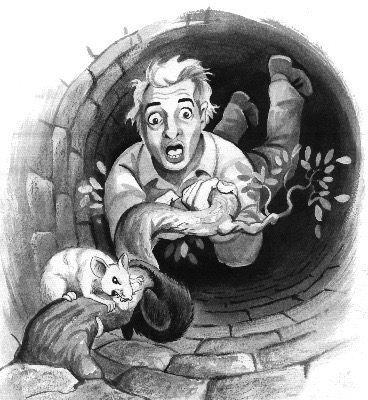
\includegraphics{/Teaching/Examined/Meaning/Tolstoy.jpg} \textgreater{}
Imagine a traveller fleeing a ferocious, hungry beast. Our traveller's
only means of escape is a well they stumble upon. They jump down to
escape the infuriated beast who remains waiting at the well's edge. Some
great trees grow beside our well, its roots jutting down and through its
walls. The traveller reaches out, grabs the roots and saves himself from
falling, which turns out quite fortuitous. As his eyes adjust, the
traveller notices red glowing eyes at the bottom of the well. A dragon!
\textgreater{} Our traveler is stuck. The beast above awaits if he
climbs up. The dragon below awaits if he climbs down. He pauses,
clutching the roots growing from the cleft of the well wall. Things get
worse. Two mice, one black and one white, appear and start nibbling on
the roots. Our traveller realizes that the roots will break and
inevitably he will fall into the dragon's jaws below. \textgreater{}
While he is still clinging, he sees some drops of honey hanging on the
roots, and so reaches out for them with his tongue. He tastes the
sweetness, which distracts him for a while from the beast above, the
dragon below, and the mice eating the roots.

This fable, says Tolstoy, depicts the life each of us live. The dragon
and beast represent death. The mice represent time. The honey represents
those things we use to distract ourselves from our mortality: family,
career, etc. These are supposed to be what give our lives internal
value, they are the things that make us think that life is choice
worthy. But would you find the honey sweet if you were in that well?
Maybe initially. But your awareness of the dragon, beast, and mice will
likely dampen, if not destroy, your continued enjoyment of the honey.
Similarly, Tolstoy suggests that none of the things we use to distract
ourselves from our mortality can continue to do so indefinitely. He
claims: \textgreater{} ``Just so I hold on to the branch of life,
knowing that the dragon of death is waiting inevitably for me, ready to
tear me to pieces, and I cannot understand why I have fallen on such
suffering. And I try to lick that honey which used to give me pleasure,
but now it no longer gives me joy, and the white and black mouse day and
night nibble at the branch to which I am holding on. I clearly see the
dragon, and the honey is no longer sweet to me. I see only the
inevitable dragon and the mice, and am unable to turn my glance away
from them. This is not a fable, but a veritable, indisputable,
comprehensible truth.'' (Tolstoy, p.12) \textgreater{} ``The deception
of the joys of life which formerly allayed my terror of the dragon now
no longer deceived me\ldots{}The two drops of honey which diverted my
eyes from the cruel truth longer than the rest: my love of family, and
of writing - art as I called it - were no longer sweet to me.''
(Tolstoy, p.12)

\begin{quote}
``Family\ldots{}said I to myself. But my family - wife and children -
are also human. They are placed just as I am: they must either live in a
lie or see the terrible truth. Why should they live? Why should I love
them, guard them, bring them up, or watch them? That they may come to
the despair that I feel, or else be stupid? Loving them, I cannot hide
the truth from them: each step in knowledge leads them to the truth. And
the truth is death\ldots{}.No sweetness of honey could be sweet to me
when I saw the dragon and saw the mice gnawing away my support.''
(Tolstoy, p.12)
\end{quote}

\begin{quote}
``It was indeed terrible. And to rid myself of the terror I wished to
kill myself. I experienced terror at what awaited me---knew that that
terror was even worse than the position I was in, but still I could not
patiently await the end. However convincing the argument might be that
in any case some vessel in my heart would give way, or something would
burst and all would be over, I could not patiently await that end. The
horror of darkness was too great, and I wished to free myself from it as
quickly as possible by noose or bullet. That was the feeling which drew
me most strongly towards suicide.'' (Tolstoy, p.13)
\end{quote}

How do these remarks prove Premises 2 and 3? Let's take each in turn.
Recall that Premise 2 states that life has internal value only if it has
external value. As a corollary, if life has no external value, then it
has no internal value. Tolstoy's argument for this claim is hard to
discern, but seems to rely on claims about human psychology:

\begin{itemize}
\item
  \begin{enumerate}
  \def\labelenumi{(\alph{enumi})}
  \itemsep1pt\parskip0pt\parsep0pt
  \item
    I will find some project/goal valuable over a long period of time,
    only if I believe that project/goal is externally valuable.
  \end{enumerate}
\item
  \begin{enumerate}
  \def\labelenumi{(\alph{enumi})}
  \setcounter{enumi}{1}
  \itemsep1pt\parskip0pt\parsep0pt
  \item
    None of my projects/goals are externally valuable.
  \end{enumerate}
\item
  \begin{enumerate}
  \def\labelenumi{(\alph{enumi})}
  \setcounter{enumi}{2}
  \itemsep1pt\parskip0pt\parsep0pt
  \item
    I will inevitably discover that my projects/goals have no external
    value.
  \end{enumerate}
\item
  \begin{enumerate}
  \def\labelenumi{(\alph{enumi})}
  \setcounter{enumi}{3}
  \itemsep1pt\parskip0pt\parsep0pt
  \item
    I will inevitably cease to find internal value in my life (from
    a-c).
  \end{enumerate}
\item
  \begin{enumerate}
  \def\labelenumi{(\alph{enumi})}
  \setcounter{enumi}{4}
  \itemsep1pt\parskip0pt\parsep0pt
  \item
    I will inevitably cease to find life choice worthy (from d)
  \end{enumerate}
\end{itemize}

Let's hold our discussion of (c) until the next section and focus on (a)
and (b). Tolstoy's doesn't do much to motivate (a), but it does seem to
apply to a large number of people. Suppose, for instance, you dedicate
your life to eradicating poverty, or writing the greatest novel, or
caring for your children.

\begin{quote}
News flash! An asteroid is heading our way. It will destroy Earth and
all life in one month's time.
\end{quote}

If this were true, many would struggle to keep working on their
projects. The poverty fighter is unlikely to stay up late at night
writing letters to congress arguing for poverty relief. The novelists
will likely put down their pens when they stumble on a difficult
passage. The parent who works 3 jobs to pay for their child's education
is going to quit.

The asteroid won't hit us in 30 days time. But Tolstoy is asking us to
really consider the fact that our death is inevitable. The poverty
fighter will give up if the people they fight for will die within a
month. Even though the sick and starving may not die in a month, they
will die. It's inevitable. Even the human species will one day be no
more.

The fact that some will outlive us is hardly a consolation. Consider the
novelist. Perhaps there are those who will read her work in 200 years
time. But 200 years is tiny blip in the history of the universe. Few
would fret over writing a novel if they knew it would be read by a few
people for a few weeks. But what does an extra few years and readers
matter? Even if your novel is read for several years after your death,
there will inevitably arrive a point when there are no humans around to
read it. Even our families will inevitably die. We fear their death. We
put huge amount of time and energy into ensuring that their death is far
away and that they enjoy the time they have. But from the perspective of
the universe, they won't live that long regardless of how long the live.
Tolstoy thinks nothing about this horrid position should make you strive
to keep your family alive any longer.

Perhaps Tolstoy is right that we only find our projects internally
valuable if we think they are externally valuable. But why does he deny
that they are externally valuable? Why does he accept (b)? While he does
not provide much detail, he assumes that a project has external value
only if that project has eternal results or, at least, contributes to
something that is eternal. Consider again the novel. Tolstoy points out
that no novel will be read until the end of time. There will eventually
be no more readers. So, he concludes that no novel could have external
value. Similarly, advancing the human race could only have external
value, according to Tolstoy, if humans could somehow live on eternally.
But, at this stage in his life, Tolstoy believes that humans will
inevitably die out. It seems futile he thinks to help them delay the
inevitable. \#\# Four Attitudes Toward Death If Tolstoy's diagnosis of
our lives is correct, then there are four attitudes we can take towards
our lives. Tolstoy argues the first three are neither sustainable or
rational, and so thinks the fourth is the only real option. Notice that
the first provides our argument for (c): 1. Ignorance: It consists in
not knowing, not understanding, that life is an evil and an absurdity.
People of this sort have yet to see the dragon that awaits them. They
have yet to see the mice gnawing the shrub by which they are hanging.
They lick the honey. They do so only for a while: something will
eventually turn their attention to the dragon and the mice. They will
then stop their licking. (Tolstoy, p.22)3. Epicureanism: while knowing
the hopelessness of life, make use meanwhile of the advantages one has,
disregarding the dragon and the mice, and licking the honey in the best
way, especially if there is much of it within reach. This, though, is an
unsustainable attitude. Many live in terrible conditions. Many have no
honey to taste. It is a mere accident, claims Tolstoy, that you have
good circumstances rather than poor, and `'the accident that has today
made me a Solomon may tomorrow make me a Solomon's slave.'' Epicureans
try but cannot ultimately forget that all these pleasures are ephemeral.
They are as easily lost as gained. Nobody can be confident that life
will always provide these distractions. (Tolstoy, p.22)

\begin{enumerate}
\def\labelenumi{\arabic{enumi}.}
\setcounter{enumi}{3}
\itemsep1pt\parskip0pt\parsep0pt
\item
  Weakness: ``It consists in seeing the truth of the situation and yet
  clinging to life, knowing in advance that nothing can come of it.
  People of this kind know that death is better than life, but not
  having the strength to act rationally - to end the deception quickly
  and kill themselves - they seem to wait for something. This is the
  escape of weakness, for if I know what is best and it is within my
  power, why not yield to what is best?'' (Tolstoy, p.23)
\item
  Suicide: ``This is the way of strength and energy. It consists in
  destroying life, when one has understood that it is an evil and an
  absurdity. A few exceptionally strong and consistent people act so.
  Having understood the stupidity of the joke that has been played on
  them, and having understood that it is better to be dead than to be
  alive, and that it is best of all not to exist, they act accordingly
  and promptly end this stupid joke.'' (Tolstoy, p.23)
\end{enumerate}

\end{document}
